\documentclass[a4paper]{article}
\usepackage[utf8]{inputenc}
\usepackage{fancyhdr}
\usepackage{geometry}
\usepackage{listings}
\usepackage{graphicx}
%\geometry{0.5in}

\usepackage{float}

\lstset{
    language=Python,
    breaklines=true,
    numbers=left,
    frame=lines
}

\pagestyle{fancyplain}

\title{System Maintenance}
\author{Harry Milne}
\date{March 2014}

\lhead{Harry Milne}
\chead{Candidate Number: 00000}
\rhead{Centre Number: 22169}

\begin{document}
\newpage
\tableofcontents

\maketitle

\section{Environment}
\label{sec:env}
\subsection{Software}
\begin{itemize}
    \item Python 2.7 and included modules
    
    \begin{itemize}
        \item SQLite3
    \end{itemize}
    
    \item Twisted 13.2.0 Python Module
    \item PyQt4 Python Module
    \item SimpleCV 1.3
    \item SQLite Database Browser
    \item Vim
    \item Sublime Text 3
\end{itemize}

\begin{table}[H]
    \centering
    \begin{tabular}{|p{4cm}|p{8cm}|}
    \hline
    \textbf{Software}                & \textbf{Usage Explanation}                                                                                                                                                                                            \\ \hline
    Python 2.7              & I used Python 2.7 instead of Python 3.* because of the superior module support that Python 2.5+ has. Also, the nature of Python itself makes it very easy to build systems quickly.                          \\ \hline
    SQLite3                 & SQLite3 was an easy database management system to use because it has little requirements for the system it is run on. This means you do not have to do any extensive configuration of any target system.      \\ \hline
    Twisted 13.2.0          & Twisted is a Python module which lets you very quickly prototype and build clients and servers, which is central to this system.                                                                             \\ \hline
    PyQt4                   & PyQt4 is a feature rich user interface development module, it handles all of the threading needed to run operations while keeping an operational interface.                                                  \\ \hline
    SimpleCV 1.3            & SimpleCV is aimed at making computer vision easy to develop, I used it in conjunction with the Raspberry Pi to recognise faces.                                                                              \\ \hline
    SQLite Database Browser & This open source software gives an easy way to visually check over your SQLite databases, this was invaluable in testing.                                                                                    \\ \hline
    Vim                     & When developing the python server script, it was easier to program it while on the server itself instead of deploying to it every time I wanted to test. This meant using a text editor that works in shell. \\ \hline
    Sublime Text 3          & This was the editor of choice while programming in a GUI environment, it has a lot of tools to help with syntax highlighting and variable naming.                                                            \\ \hline
    \end{tabular}
\end{table}

\section{System Overview}
The system has 3 main components; the client, server and database browser. The server and client are directly related
whereas the database browser is a `tool' I have bundled to help the user manage the database. The database browser works
with the server on a local level, in that you edit the same file on the same system that the server does. However,
the database browser requires the server to be running a graphical user environment because it is a graphical representation
of the database. 

\subsection{Client}
The client uses the SimpleCV package as shown in section~\ref{sec:env}, this package handles everything around the camera,
this makes it easier to read what is happening with the data being handled by the Python.  

\subsection{Server}


\subsection{Database Browser}

\section{Code Structure}
I structured the code so that each section of the system was an object, abstracting like this helps a lot with
visualising the code. By doing this I have taken one of the advantage of object-oriented programming; the ability
to abstract certain situations into particular `objects'.

\subsection{Client Class}
The class created in `client.py', which can be found in section~\ref{sec:client.py}, includes methods to handle
!needs updating

\subsection{Handler Class}
The server class created in `server.py' is called `Handler' as shown in section~\ref{sec:server.py} line 8, this is because it `handles' the requests from the
client. Inside this class there is an `SQLInterface' instantiation to give the server an interface for the `SQLite3'
database, however, methods that edit the database will only be run after the server knows the user trying to access
it is already in it. Unfortunately, there is no other security around authenticating users, the only barrier between
someone sending a string to the server and gaining access is that they don't know the users already in the database.


\subsection{SQLInterface Class}
I structured it this way so that if one needed to access the database from another Python script, they'd
have a standardised method of doing so. This means they can simply import the package and either instantiate it `as is'
or use it as a parent class to add functionality.

\section{Variable Listing}
\section{System Evidence}
\subsection{User Interface}
\subsection{ER Diagram}
\begin{center}
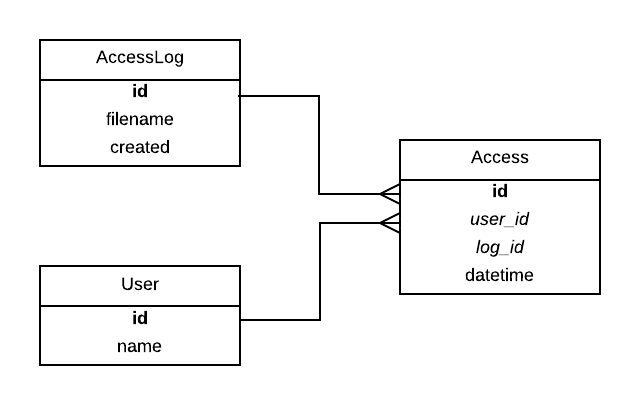
\includegraphics[scale=0.3]{../shared_assets/diagrams/ERD.png}
\end{center}

\subsection{Database Table Views}
\subsubsection{Users}
\subsubsection{Access}
\subsubsection{LogFile}

\subsection{Database SQL}

\lstinputlisting[language=Python, 
                firstline=32, 
                lastline=56, 
                caption=Extract from sql\_interface.py]{../../code/server/sql_interface.py}
Above, in Listing 1, you can see the function inside the `SQLInterface' class which creates the tables
within the database. This function \textit{must} be ran before any other inside the class if the database
hasn't been initialised before, otherwise an exception will be thrown saying either that the database 
doesn't exist yet or the tables don't exist.

The structure of this function has been coded with the `DRY' (`Don't Repeat Yourself') principle in mind;
instead of running each SQL statement individually, the strings are in a list which can be iterated over.

\subsection{SQL Queries}

\begin{table}[H]
    \centering
    \begin{tabular}{|p{5cm}|p{8cm}|}
    \hline
    \textbf{Functionality}                                                                                                                   & \textbf{SQL Statement}                                                                                                                                          \\ \hline
    Creates a new User with the given user\_name.                                                                   & INSERT INTO Users(user\_name) values (?)                                         \\ \hline
    Delete a user with a given id.                                                                                  & DELETE FROM Users where user\_id = ?                                             \\ \hline
    Return all stored user\_name attributes in the Users table.                                                     & SELECT user\_name FROM Users                                                     \\ \hline
    Return all Users entities with the given user\_name.                                                            & SELECT * from Users WHERE user\_name = ?                                         \\ \hline
    Return the Users entity with the given user\_id.                                                                & SELECT user\_name FROM Users WHERE user\_id = ?                                  \\ \hline
    Create new Log entity with the given filename and created date.                                                 & INSERT INTO Log(log\_filen, log\_created) VALUES (?,?)                           \\ \hline
    Return the Log with the highest id number.                                                                      & SELECT * FROM Log WHERE log\_id=(SELECT MAX(log\_id) FROM Log)                   \\ \hline
    Create an entity in the Access table with the given attributes; user\_id, log\_id, access\_date and access\_toggle. & INSERT INTO Access(user\_id, log\_id, access\_date, access\_toggle) VALUES (?,?,?,?) \\ \hline
    Return all Access entities initiated with the given user\_id.                                                   & SELECT * FROM Access WHERE user\_id = ?                                          \\ \hline
    \end{tabular}
\end{table}

\section{Testing}
\subsection{Summary of Results}
\subsection{Known Issues}
\section{Code Explanations}
\subsection{Difficult Sections}
\begin{itemize}
    \item Learning SimpleCV
    \item Learning Twisted
    \item Handling Physical Log Files
    \item Editing an existing project
\end{itemize}
\subsection{Self-created Algorithms}
\section{Settings}
\subsection{Server}
The server has it's settings contained in a `.cfg' file, which is placed in the same directory as `main.py',
the system uses a Python object called `ConfigParser' which reads from this plain-text file and stores it in
the object.
\lstinputlisting[caption=server.cfg]{../../code/server/server.cfg}

\subsection{Client}
\ref{sec:client.py}
%\lstinputlisting{../../code/client/client.cfg}
\section{Acknowledgements}
\subsection{Adam McNicol}
The code I used to create the Database Browser was forked from the repository from github.com/MrAGi, I trimmed
down the original code and edited things like the file browser to more suit my needs. Taking advantage of
open source projects is a great way of saving time and learning from other peoples code. After seeing the code
in use before, it seemed logical to just take that project and change it slightly to fit my project. The best
thing about it was that it was already very well tested since the entire class had already been using it without
any problems.

\subsection{Code Listing Appendix}
\newpage
\subsubsection{client/client.py}
\label{sec:client.py}
\lstinputlisting{../../code/client/client.py}

\subsubsection{server/main.py}
\label{sec:main.py}
\lstinputlisting{../../code/server/main.py}

\subsubsection{server/server.py}
\label{sec:server.py}
\lstinputlisting{../../code/server/server.py}

\subsubsection{server/sql\_interface.py}
\label{sec:sqlinterface.py}
\lstinputlisting{../../code/server/sql_interface.py}

\subsubsection{db\_browser/db\_browser.pyw}
\label{sec:dbbrowser.py}
\lstinputlisting{../../code/db_browser/db_browser.pyw}

\subsubsection{db\_browser/dialogs.py}
\label{sec:dialogs.py}
\lstinputlisting{../../code/db_browser/dialogs.py}

\subsubsection{db\_browser/sqlite\_browse\_data.py}
\label{sec:browsedata.py}
\lstinputlisting{../../code/db_browser/sqlite_browse_data.py}

\subsubsection{db\_browser/sqlite\_connection.py}
\label{sec:connection.py}
\lstinputlisting{../../code/db_browser/sqlite_connection.py}


\end{document}
